
\chapter{Inference for categorical data}
\label{inferenceForCategoricalData}



In 1945, the United States was at war with Japan in World War II, and
it had secretly developed a new weapon: an atomic bomb. The decision
to use that device was a difficult one, but on August 6th, the United
States dropped an atomic bomb on Hiroshima, Japan, killing at least
66,000 people. Opinions vary on if it was it the right choice to use
the atomic bomb. Seventy years later in 2015, Pew Research conducted
a poll that found that 56\% of Americans believed the use of nuclear
weapons was justified.\footnote{
\oiRedirect{textbook-pew_2015_poll_on_hiroshima}{http://www.pewglobal.org/2015/04/07/survey-methods-67/}}
\Comment{The redirect link in the footnote needs to be confirmed as
working.}
This poll was based on a simple random sample of 1,000 American
adults.
\begin{quote}
If the poll was based on only 1,000 people, how reliable is it?
\end{quote}
If we took another poll, we wouldn't get the exact same answer.
Ultimately, it's unlikely that the actual proportion of Americans
who believe the use of nuclear weapons is \emph{exactly} 56\%,
but it's probably something close to 56\%.

Statistical inference is concerned primarily with understanding the
accuracy of parameter estimates. While the equations and details change
depending on the setting, the foundations for inference are the same
throughout all of statistics. We introduce these common themes in
Sections~\ref{pointEstimates}-\ref{} by discussing inference about the
population proportion, $p$, and we'll expand on these ideas into other
context in later chapters.


%__________________
\section[Point estimates and sampling variability]{Point estimates and
sampling variability} %\sectionvideohref{youtube-DNIauUrRIEM&list=PLkIselvEzpM7Pjo94m1e7J5jkIZkbQAl4}~\sectionslideshref{gdoc_os3_slides_4-1}}
\label{pointEstimates}

In 2015, a Pew Research poll of 1,000 American adults found that
56\% believed the use of nuclear weapons was justified.
In this section, we discuss what a point estimate like 56\% represents
and the uncertainty we have associated with such estimates. We'll also
be using some new notation:
\begin{itemize}
\item The population proportion will be written as $p$.
\item When we look at the proportion computed from the sample,
    it will have a label $\hat{p}$ (spoken as \emph{p-hat}).
\item The size of a sample will generally be denoted by $n$.
\end{itemize}
In the Pew Study, we know the sample proportion is
$\hat{p} = 0.56$ and $n = 1000$. Typically we do not know the
population proportion $p$, and we use the sample data to
understand what possible values of $p$ are plausible.

\subsection{Point Estimates}
\label{pointEstimates}

\index{point estimate|(}

The poll provides a \term{point estimate} of the actual proportion
of American adults that believe the use of nuclear weapons was
justified. This estimate of 56\% is unlikely to be perfect, and
it's quite possible for the \term{true proportion}
(a.k.a. the population proportion) to be a little lower
or a little higher. The difference between a point estimate and
the actual value it tries to estimate is called the estimate's
\term{error}.

The error varies from one sample to the next: maybe
in one sample it is 1\% too low while in another
it is 2\% too high. Unfortunately, we rarely know the direction
or size of the error in our estimates, so instead we focus
on understanding what kinds of errors are typical.


\subsection{Simulation to understand variability}

Let's step back a moment and pretend that the population proportion
was $p = 0.56$. If we took a random sample from this population, how
accurate would the point estimate be? Here's how we might simulate it:
\begin{enumerate}
\item There were about 247 million American adults in 2015. Retrieve
    247 million pieces of paper, and write ``justified'' on 56\% of
    them and ``not'' on 44\% of them.
\item Mix up the pieces of paper and pull out 1000 pieces.
\item Compute the fraction of those 1000 pieces that say ``justified''.
\end{enumerate}
Any volunteers to conduct this simulation? Probably not. Running
this simulation with 247 million pieces of paper would be
time-consuming and costly, but we can simulate it
using computer code; we've written a short program in the
footnote.\footnote{Code using the statistical software called \R: \\
\texttt{\# 1. Create a set of 247 million entries,
where 56\% of them are "justified" and 44\% are "not". \\
possible\_entries <- rep(c("justified", "not"), c(0.56, 0.44) * 247e6)\\
\# 2. Sample 1000 of the entries. \\
sampled\_entries <- sample(possible\_entries, 1000) \\
\# 3. Count the number that are "justified", then divide
by the sample size. \\
sum(sampled\_entries == "justified") / 1000}}
After running the simulation, we got an estimate
of $\hat{p}_1 = 0.575$. We know the population proportion
is $p = 0.56$, so we know the estimate had an error of +0.015.
%We only know this error because we know the population proportion,
%which is very rarely the case and would defeat the need for a sample
%in a real-world setting.

One simulation isn't enough to get a sense of the null
distribution, so we should repeat the simulation. In a second
simulation, we get $\hat{p}_2 = 0.585$, which has an error of
+0.025.
In another, $\hat{p}_3 = 0.54$ for an error of -0.02. And in another,
an estimate of $\hat{p}_4 = 0.556$ with an error of -0.004.
With the help of a computer, we've run the simulation 10,000 times
and create a histogram of the sample proportions from the simulation
in Figure~\ref{sampling_10k_prop_56p}. This
distribution of sample proportion is called a
\term{sampling distribution}. In real-world applications,
\emph{we never actually observe the sampling distribution, yet we
should always think of the sample proportion as coming from
such a distribution}.
%\footnote{Here is the code for 10,000 simulations: \\
%\texttt{people <- rep(c("justified", "not"), c(0.56, 0.44) * 247e6) \\
%sim.results <- c() \\
%for (i in 1:10000) \{ \\
%\ \hspace{5mm}sampled.people <- sample(people, 1000) \\
%\ \hspace{5mm}sim.results[i] <- mean(sampled.people == "justified") \\
%\} \\
%hist(sim.results, 20)} \\
%(There's actually a more efficient way to write this code, but we have provided you the long version!)}
We can characterize this sampling distribution as follows:
\begin{description}
\item[Center.] The center of the distribution is
    $\bar{x}_{\hat{p}} = 0.56$, which is the same as the
    population proportion.
    In~other words, the sample proportion is an
    \term{unbiased estimate} of the population proportion.
\item[Spread.] The standard deviation of the distribution
    is $s_{\hat{p}} = 0.0157$. When we're talking about
    a sampling distribution or the variability of
    a point estimate, we typically use the term
    \term{standard error} rather than \emph{standard deviation}
    and use the notation $SE_{\hat{p}}$ for the standard
    error associated with the sample proportion.
\item[Shape.] The distribution is symmetric and bell-shaped,
    and it \emph{resembles a normal distribution}.
\item[Unusual characteristics.] There aren't any obvious outliers.
\end{description}
These findings are very encouraging! When the population
proportion is $p = 0.56$ and the sample size is $n = 1000$,
the sample proportion $\hat{p}$ tends to give a pretty good estimate
of the population proportion. We also have this interesting observation
that the histogram resembles a normal distribution.

\begin{figure}
   \centering
   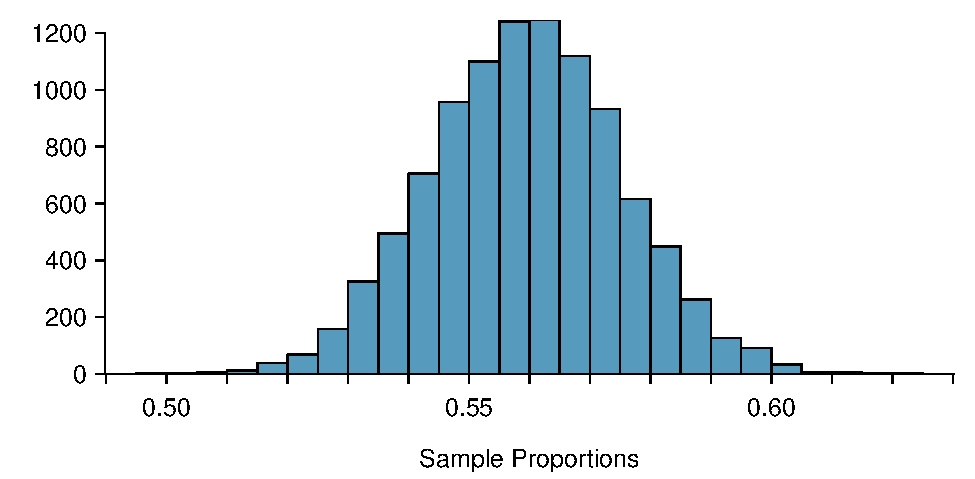
\includegraphics[width=0.8\textwidth]{ch_inference_for_props/figures/sampling_10k_prop_56p/sampling_10k_prop_56p}
   \caption{A histogram of 10,000 sample proportions, where each
       sample is taken from a population where the population of
       proportion is 0.56 and the sample size is $n = 1000$.}
   \label{sampling_10k_prop_56p}
\end{figure}

\begin{example}{If we used a much smaller sample size of $n = 50$,
would you guess that the standard error for $\hat{p}$ would be larger
or smaller than when we used $n = 1000$?}
\label{smallerSampleWhatHappensToPropErrorExercise}
Intuitively, it seems like more data is better
than less data, and generally that is correct! The typical error
when $p = 0.56$ and $n = 50$ would be larger
than the error we would expect when $n = 1000$.
\end{example}

\noindent
Example~\ref{smallerSampleWhatHappensToPropErrorExercise}
highlights an important property: bigger samples
tend to be more precise than smaller samples.

\index{point estimate|)}


\subsection{Central Limit Theorem}

The distribution in
Figure~\ref{sampling_10k_prop_56p} looks an awful lot like
a normal distribution. That is no anomaly; it is the result
of a general principle called the \term{Central Limit Theorem}.
\index{Central Limit Theorem!proportion|textbf}

\begin{termBox}{\tBoxTitle{Central Limit Theorem for proportions
    \& the success-failure condition}
When the observations are independent and the sample size is
sufficiently large, the sample proportion $\hat{p}$ will tend
to follow a normal distribution with the following mean and
standard error:
\begin{align*}
  \mu_{\hat{p}} &= p
  &SE_{\hat{p}} &= \sqrt{\frac{p (1 - p)}{n}}
\end{align*}
The sample size is typically considered sufficiently large when
$np \geq 10$ and $n(1-p) \geq 10$, which is called the
\term{success-failure condition}.} %since $np$ represents the
%number of expected \emph{successes} and $n(1-p)$ the expected
%number of \emph{failures}.}
\end{termBox}

The Central Limit Theorem is incredibly important, and it provides
a foundation for the rest of this book. As we begin applying
this principle, be mindful of the two requirements:
the observations must be independent, and the the sample size must
be sufficiently large such that $np \geq 10$ and $n(1-p) \geq 10$.

\begin{example}{Earlier we estimated the mean and standard
deviation of the $\hat{p}$'s using simulated data when $p = 0.56$
and $n = 1000$. Confirm that the distribution is approximately
normal.}\label{sample_p56_n1000_confirm_normal}
\begin{description}
\item[Independence.] There are $n = 1000$ observations for each
    sample proportion $\hat{p}$, and each of those observations
    are independent draws. \emph{The most common way for
    observations to be considered independent is if they are from
    a simple random sample.}
    \index{independent}
    \index{independence}
    \index{Central Limit Theorem|independence}
\item[Success-failure condition.] We can confirm the sample size
    is sufficiently large by checking the success-failure condition
    and confirming each of the following values are greater than 10:
    \begin{align*}
    np &= 1000 \times 0.56 = 560
    &n(1-p) &= 1000 \times (1 - 0.56) = 440
    \end{align*}
\end{description}
Both of the independence and success-failure conditions are
satisfied, so the Central Limit Theorem applies and the normal
distribution is reasonable in this context!
\end{example}

\begin{example}{Compute the theoretical mean and standard deviation
of the $\hat{p}$'s when $p = 0.56$ and $n = 1000$, according to the
Central Limit Theorem.}\label{sample_p56_n1000_mean_se}
The mean of the $\hat{p}$'s is simply the population proportion:
$\mu_{\hat{p}} = 0.56$.

The calculation of the standard error of $\hat{p}$ uses
the following formula:
\begin{align*}
SE_{\hat{p}}
    = \sqrt{\frac{p (1 - p)}{n}}
    = \sqrt{\frac{0.56 (1 - 0.56)}{1000}}
    = 0.0157
\end{align*}
\end{example}

\begin{example}{Estimate how frequently the sample proportion
$\hat{p}$ should be within 0.02 (2\%) of the population value,
$p = 0.56$. Based on Examples~\ref{sample_p56_n1000_confirm_normal}
and~\ref{sample_p56_n1000_mean_se}, we know that the distribution
is $N(\mu_{\hat{p}} = 0.56, SE_{\hat{p}} = 0.0157)$.}
\label{sampling_10k_prop_56p-prop_from_53_to_59}
After so much practice in Section~\ref{normalDist},
this example will hopefully feel familiar!
We would like to understand the fraction of $\hat{p}$'s
between 0.54 and 0.58:
\begin{center}
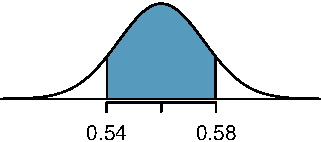
\includegraphics[width=60mm]{ch_inference_for_props/figures/p-hat_from_54_and_58/p-hat_from_54_and_58}
\end{center}
With $\mu_{\hat{p}} = 0.56$ and $SE_{\hat{p}} = 0.0157$,
we can compute the Z-score for both the left and right cutoffs:
\begin{align*}
Z_{0.54} &= \frac{0.54 - 0.56}{0.0157} = -1.27
&Z_{0.58} &= \frac{0.58 - 0.56}{0.0157} = 1.27
\end{align*}
We can use either statistical software, a graphing calculator,
or a table to find the areas to the tails, and in any case we
will find that they are each 0.1020. The total tail areas are
$2 \times 0.1020 = 0.2040$, which leaves the shaded area of
0.7960. That is, about 79.6\% of the sampling distribution
in Figure~\ref{sampling_10k_prop_56p} is within $\pm0.02$
of the population proportion, $p = 0.56$.
%of these
%cutoffs and compute the difference of these areas
%to get the central area:
%\begin{center}
%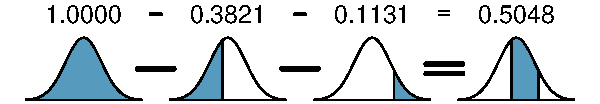
\includegraphics[width=60mm]{ch_inference_for_props/figures/p-hat_from_53_and_59_computation/p-hat_from_53_and_59_computation}
%\end{center}
\end{example}

\begin{exercise}
In Example~\ref{smallerSampleWhatHappensToPropErrorExercise}
we discussed how a smaller sample would tend
to produce a less reliable estimate. Explain how this intuition
is reflected in the formula for
$SE_{\hat{p}} = \sqrt{\frac{p (1 - p)}{n}}$.\footnote{Since the
sample size $n$ is in the denominator of the fraction (on the
bottom of the fraction), a bigger sample size means the entire
expression when calculated will tend to be smaller. That is,
a larger sample size would correspond to a smaller standard error.}
\end{exercise}

%In Example~\ref{sampling_10k_prop_56p}, we applied a general
%principle called the \term{Central Limit Theorem}
%\hiddenterm{Central Limit Theorem!proportions} when
%we used the normal distribution as an approximation.


\subsection{Applying the Central Limit Theorem to a real-world setting}

Think back to the 2015 poll where
$\hat{p} = 0.56$ of American adults believed the use of nuclear
weapons in WW2 was justified. We might wonder: does the sample
proportion from the poll approximately follow a normal
distribution? We check the conditions from the Central
Limit Theorem:
\begin{description}
\item[Independence.] The poll is a simple random sample of
    American adults, which means that the observations are
    independent.
\item[Success-failure condition.] To check this condition,
    we need the population proportion, $p$, to check if both
    $np$ and $n(1-p)$ are greater than 10. However, we do not
    know the value of $p$; that's exactly why the pollsters
    took a sample! In cases like these, we use $\hat{p}$ as
    our next best way to check the success-failure condition:
    \begin{align*}
    n\hat{p} &= 1000 \times 0.56 = 560
    &n (1 - \hat{p}) &= 1000 \times (1 - 0.56) = 440.
    \end{align*}
    While we cannot check the condition with $p$,
    $\hat{p}$ acts as a reasonable substitute.
\end{description}

This \term{substitution approximation} of using $\hat{p}$ in
place of $p$ can also be used when computing the standard error
of the sample proportion:
\begin{align*}
SE_{\hat{p}}
    = \sqrt{\frac{p (1 - p)}{n}}
    \approx \sqrt{\frac{\hat{p} (1 - \hat{p})}{n}}
    = 0.0157
\end{align*}

Unfortunately this substitution approximation doesn't always work.
While it will be reasonable for working with proportions
throughout this chapter,\footnote{There are additional methods
for proportions that perform some correction for the substitution
approximation. However, we leave those proportion methods for
a future course.}
we will find that the approximation cannot always be trusted
when we work with sample means in
Chapter~\ref{inferenceForNumericalData}.



%__________________
\section[Confidence intervals]{Confidence intervals} % \sectionvideohref{youtube-FUaXoKdCre4&list=PLkIselvEzpM7Pjo94m1e7J5jkIZkbQAl4}~\sectionslideshref{gdoc_os3_slides_4-2}}
\label{confidenceIntervals}

\index{confidence interval|(}

A point estimate provides a single plausible value for
a parameter, e.g. the population proportion of interest.
However, no point estimate is perfect, and
each point estimate will have some \emph{standard error}
associated with it. Instead of supplying just a point
estimate of a parameter, a next logical step would be
to provide a plausible \emph{range of values} for the
parameter.

\subsection{Capturing the population parameter}

A plausible range of values for the population parameter
is called a \term{confidence interval}.

Using only a point estimate is like fishing in a murky
lake with a spear, and using a confidence interval is
like fishing with a net. We can throw a spear where we
saw a fish, but we will probably miss. On the other hand,
if we toss a net in that area, we have a good chance of
catching the fish.

If we report a point estimate $\hat{p}$, we probably
will not hit the exact population proportion. On the
other hand, if we report a range of plausible values
-- a confidence interval -- we have a good shot at
capturing the parameter. 

\begin{exercise}
If we want to be very certain we capture the population
proportion in an interval, should we use a wider interval
or a smaller interval?\footnote{If we want to be more
certain we will capture the fish, we might use a
wider net. Likewise, we use a wider confidence interval
if we want to be more certain that we capture the
parameter.}
\end{exercise}

\subsection{An approximate 95\% confidence interval}

Our point estimate is the most plausible value of the parameter, so it makes sense to build the confidence interval around the point estimate. The standard error, which is a measure of the uncertainty associated with the point estimate, provides a guide for how large we should make the confidence interval.

The standard error represents the standard deviation associated with the estimate, and roughly 95\% of the time the estimate will be within 2 standard errors of the parameter. If~the interval spreads out 2 standard errors from the point estimate, we can be roughly 95\% \term{confident} that we have captured the true parameter:
\begin{eqnarray}
\text{point estimate}\ \pm\ 2\times SE
\label{95PercentConfidenceIntervalFormula}
\end{eqnarray}
But what does ``95\% confident'' mean? Suppose we took many samples and built a confidence interval from each sample using Equation~(\ref{95PercentConfidenceIntervalFormula}). Then about 95\% of those intervals would contain the actual mean, $\mu$. Figure~\ref{95PercentConfidenceInterval} shows this process with 25 samples, where 24 of the resulting confidence intervals contain the average number of days per week that YRBSS students are physically active, $\mu=3.90$~days, and one interval does not.

\begin{figure}[b]
   \centering
   %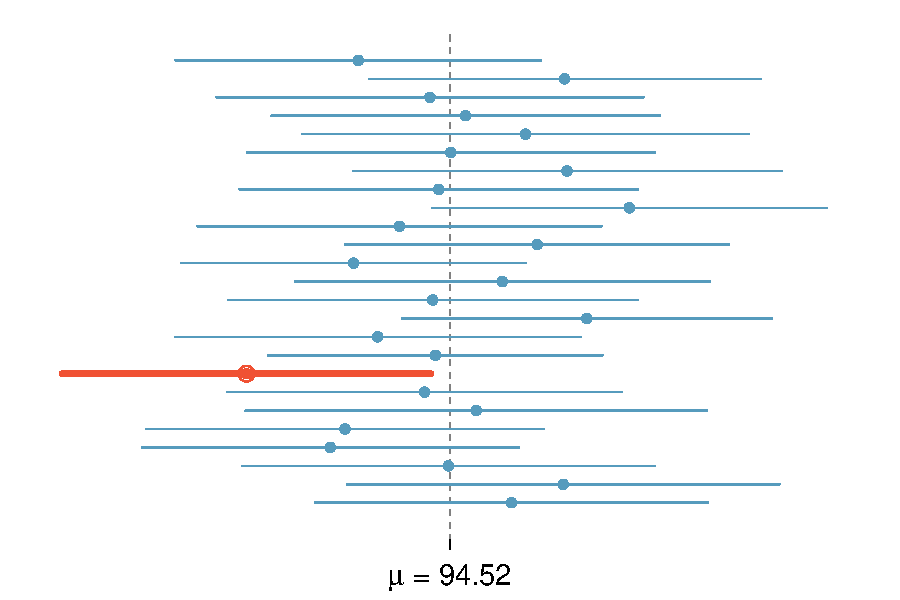
\includegraphics[width=0.78\textwidth]{ch_inference_foundations/figures/95PercentConfidenceInterval/95PercentConfidenceInterval}
   \caption{Twenty-five samples of size $n=100$ were taken from \data{yrbss}. For~each sample, a confidence interval was created to try to capture the average number of days per week that students are physically active. Only~1 of these~25 intervals did not capture the true mean, $\mu = 3.90$~days.}
   \label{95PercentConfidenceInterval}
\end{figure}

\begin{exercise}
In Figure~\ref{95PercentConfidenceInterval}, one interval does not contain 3.90 days. Does this imply that the mean cannot be 3.90?\footnote{Just as some observations occur more than 2 standard deviations from the mean, some point estimates will be more than 2 standard errors from the parameter. A confidence interval only provides a plausible range of values for a parameter. While we might say other values are implausible based on the data, this does not mean they are impossible.}
\end{exercise}

The rule where about 95\% of observations are within 2 standard deviations of the mean is only approximately true. However, it holds very well for the normal distribution. As we will soon see, the mean tends to be normally distributed when the sample size is sufficiently large. 

\begin{example}{The sample mean of days active per week from \data{yrbss\_samp} is 3.75~days. The standard error, as estimated using the sample standard deviation, is $SE=\frac{2.6}{\sqrt{100}} = 0.26$~days. (The population SD is unknown in most applications, so we use the sample SD here.) Calculate an approximate 95\% confidence interval for the average days active per week for all YRBSS students.}
We apply Equation~(\ref{95PercentConfidenceIntervalFormula}):
\begin{eqnarray*}
3.75\ \pm\ 2 \times  0.26 \quad \rightarrow \quad (3.23, 4.27)
\end{eqnarray*}
Based on these data, we are about 95\% confident that the average days active per week for all YRBSS students was larger than 3.23 but less than 4.27~days. Our~interval extends out 2 standard errors from the point estimate, $\bar{x}_{active}$.
\end{example}
% library(openintro); library(xtable); d <- yrbss.samp; mean(d$physically_active_7d); sd(d$physically_active_7d); sd(yrbss$physically_active_7d, na.rm=TRUE)

\begin{exercise} \label{95CIExerciseForAgeOfYrbssSamp1}
The sample data suggest the average YRBSS student height is $\bar{x}_{height} = 1.697$ meters with a standard error of 0.0088 meters (estimated using the sample standard deviation, 0.088 meters). What is an approximate 95\% confidence interval for the average height of all of the YRBSS students?\footnote{Apply Equation~(\ref{95PercentConfidenceIntervalFormula}): $1.697 \ \pm \ 2\times 0.0088 \rightarrow (1.6794, 1.7146)$. We interpret this interval as follows: We are about 95\% confident the average height of all YRBSS students was between 1.6794 and 1.7146 meters (5.51~to 5.62~feet).}
\end{exercise}
% library(openintro); d <- yrbss.samp; mean(d$height); sd(d$height)

\subsection{The sampling distribution for the mean}

In Section~\ref{seOfTheMean}, we introduced a sampling distribution for $\bar{x}$, the average days physically active per week for samples of size 100. We examined this distribution earlier in Figure~\ref{yrbssActive1000SampDist}. Now we'll take 100,000 samples, calculate the mean of each, and plot them in a histogram to get an especially accurate depiction of the sampling distribution. This histogram is shown in the left panel of Figure~\ref{yrbssActiveBigSampDist}.

\begin{figure}
   \centering
   %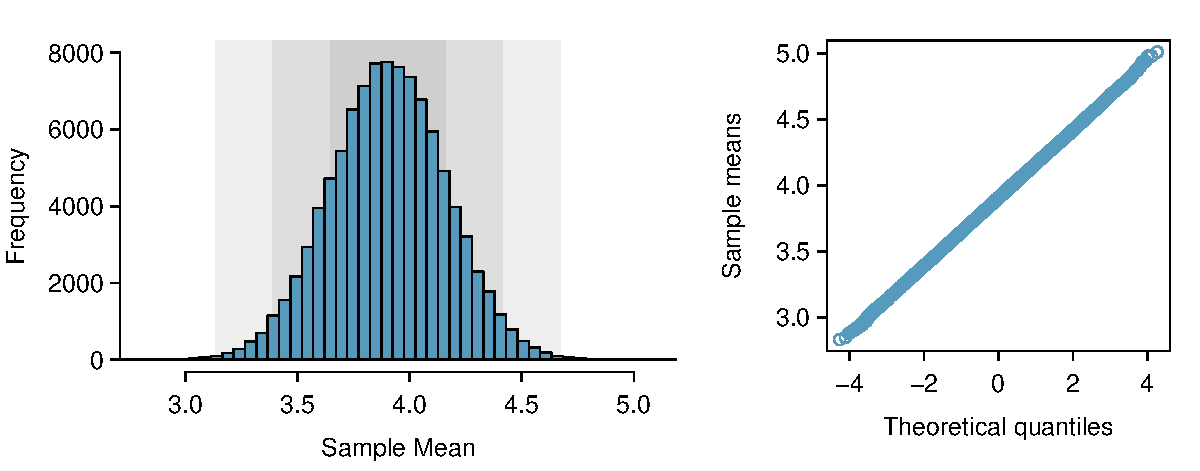
\includegraphics[width=\textwidth]{ch_inference_foundations/figures/yrbssActiveBigSampDist/yrbssActiveBigSampDist}
   \caption{The left panel shows a histogram of the sample means for 100,000 different random samples. The right panel shows a normal probability plot of those sample means.}
   \label{yrbssActiveBigSampDist}
\end{figure}

Does this distribution look familiar? Hopefully so! The distribution of sample means closely resembles the normal distribution (see Section~\ref{normalDist}). A normal probability plot of these sample means is shown in the right panel of Figure~\ref{yrbssActiveBigSampDist}. Because all of the points closely fall around a straight line, we can conclude the distribution of sample means is nearly normal. This result can be explained by the Central Limit Theorem.

\begin{termBox}{\tBoxTitle{Central Limit Theorem, informal description}
If a sample consists of at least 30 independent observations and the data are not strongly skewed, then the distribution of the sample mean is well approximated by a~normal model.\index{Central Limit Theorem}}
\end{termBox}

We will apply this informal version of the Central Limit Theorem for now, and discuss its details further in Section~\ref{cltSection}.

The choice of using 2 standard errors in Equation~(\ref{95PercentConfidenceIntervalFormula}) was based on our general guideline that roughly 95\% of the time, observations are within two standard deviations of the mean. Under the normal model, we can make this more accurate by using 1.96 in place~of~2.
\begin{eqnarray}
\text{point estimate}\ \pm\ 1.96\times SE
\label{95PercentCIWhenUsingNormalModel}
\end{eqnarray}
If a point estimate, such as $\bar{x}$, is associated with a normal model and standard error $SE$, then we use this more precise 95\% confidence interval.


\subsection{Changing the confidence level}
\label{changingTheConfidenceLevelSection}

\index{confidence interval!confidence level|(}

Suppose we want to consider confidence intervals where the confidence level is somewhat higher than 95\%; perhaps we would like a confidence level of 99\%. Think back to the analogy about trying to catch a fish: if we want to be more sure that we will catch the fish, we should use a wider net. To create a 99\% confidence level, we must also widen our 95\% interval. On the other hand, if we want an interval with lower confidence, such as 90\%, we could make our original 95\% interval slightly slimmer.

The 95\% confidence interval structure provides guidance in how to make intervals with new confidence levels. Below is a general 95\% confidence interval for a point estimate that comes from a nearly normal distribution:
\begin{eqnarray}
\text{point estimate}\ \pm\ 1.96\times SE
\end{eqnarray}
There are three components to this interval: the point estimate, ``1.96'', and the standard error. The choice of $1.96\times SE$ was based on capturing 95\% of the data since the estimate is within 1.96 standard deviations of the parameter about 95\% of the time. The choice of 1.96 corresponds to a 95\% confidence level. 

\begin{exercise} \label{leadInForMakingA99PercentCIExercise}
If $X$ is a normally distributed random variable, how often will $X$ be within 2.58 standard deviations of the mean?\footnote{This is equivalent to asking how often the Z-score will be larger than -2.58 but less than 2.58. (For a picture, see Figure~\ref{choosingZForCI}.) To determine this probability, look up -2.58 and 2.58 in the normal probability table (0.0049 and 0.9951). Thus, there is a $0.9951-0.0049 \approx 0.99$ probability that the unobserved random variable $X$ will be within 2.58 standard deviations of $\mu$.}
\end{exercise}

To create a 99\% confidence interval, change 1.96 in the 95\% confidence interval formula to be $2.58$. Guided Practice~\ref{leadInForMakingA99PercentCIExercise} highlights that 99\% of the time a normal random variable will be within 2.58 standard deviations of the mean. This approach -- using the Z-scores in the normal model to compute confidence levels -- is appropriate when $\bar{x}$ is associated with a normal distribution with mean $\mu$ and standard deviation $SE_{\bar{x}}$. Thus, the formula for a 99\% confidence interval is
\begin{eqnarray}
\bar{x}\ \pm\ 2.58\times SE_{\bar{x}}
\label{99PercCIForMean}
\end{eqnarray}

\begin{figure}
\centering
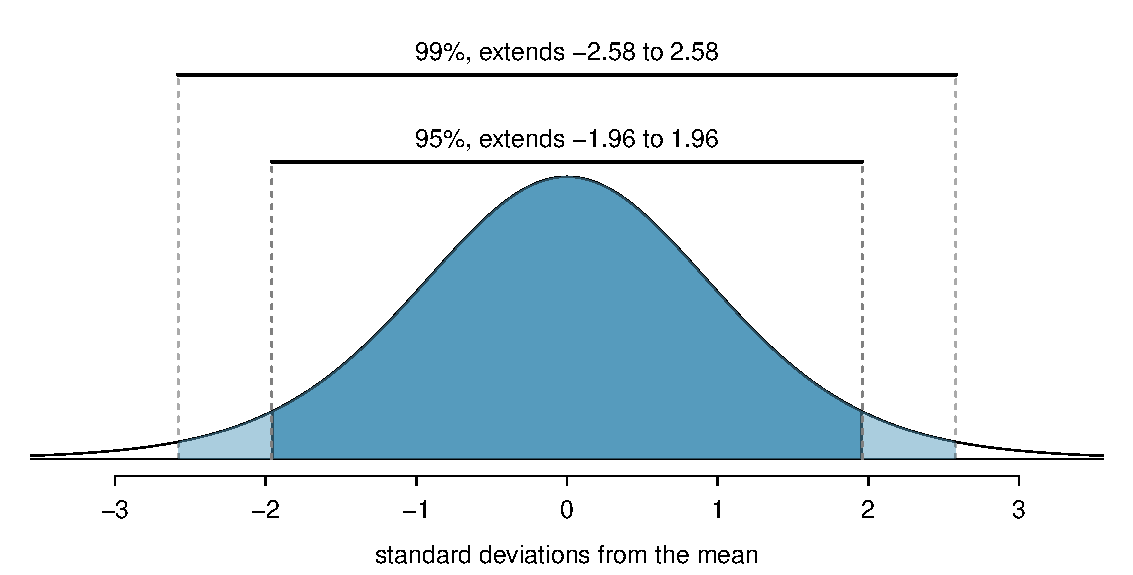
\includegraphics[width=\textwidth]{ch_inference_for_props/figures/choosingZForCI/choosingZForCI}
\caption{The area between -$z^{\star}$ and $z^{\star}$ increases as $|z^{\star}|$ becomes larger. If the confidence level is 99\%, we choose $z^{\star}$ such that 99\% of the normal curve is between -$z^{\star}$ and $z^{\star}$, which corresponds to 0.5\% in the lower tail and 0.5\% in the upper tail: $z^{\star}=2.58$.}
\label{choosingZForCI}
\index{confidence interval!confidence level|)}
\end{figure}

The normal approximation is crucial to the precision of these confidence intervals. Section~\ref{cltSection} provides a more detailed discussion about when the normal model can safely be applied. When the normal model is not a good fit, we will use alternative distributions that better characterize the sampling distribution.

\begin{termBox}{\tBoxTitle{Conditions for $\bar{x}$ being nearly normal and $SE$ being accurate\label{terBoxOfCondForXBarBeingNearlyNormalAndSEBeingAccurate}}
Important conditions to help ensure the sampling distribution of $\bar{x}$ is nearly normal and the estimate of SE sufficiently accurate:
\begin{itemize}
\setlength{\itemsep}{0mm}
\item The sample observations are independent.
\item The sample size is large: $n\geq30$ is a good rule of thumb.
\item The population distribution is not strongly skewed. This condition can be difficult to evaluate, so just use your best judgement.
\end{itemize}
Additionally, the larger the sample size, the more lenient we can be with the sample's skew.}
\end{termBox}

\begin{tipBox}{\tipBoxTitle[]{How to verify sample observations are independent}
If the observations are from a simple random sample and consist of fewer than 10\% of the population, then they are independent.\\[2mm]
Subjects in an experiment are considered independent if they undergo random assignment to the treatment groups. \\[2mm]
If a sample is from a seemingly random process, e.g. the lifetimes of wrenches used in a particular manufacturing process, checking independence is more difficult. In~this case, use your best judgement.}
\end{tipBox}

\begin{tipBox}{\tipBoxTitle[]{Checking for strong skew usually means checking for obvious outliers}
When there are prominent outliers present, the sample should contain at least 100 observations, and in some cases, much more. \\[2mm]
This is a first course in statistics, so you won't have perfect judgement on assessing skew. That's okay. If you're in a bind, either consult a statistician or learn about the studentized bootstrap (bootstrap-t) method.}
\end{tipBox}

% WARNING !!!!
% EOCE 4.9 (as of 2nd Edition) references the results of this exercise
\begin{exercise} \label{find99CIForYrbssAgeExercise}
Create a 99\% confidence interval for the average days active per week of all YRBSS students using \data{yrbss\_samp}. The point estimate is $\bar{x}_{active} = 3.75$ and the standard error is $SE_{\bar{x}} = 0.26$.\footnote{The observations are independent (simple random sample, $<10\%$ of the population), the sample size is at least 30 ($n = 100$), and the distribution doesn't have a clear skew (Figure~\ref{yrbssSampHistograms} on page~\pageref{yrbssSampHistograms}); the normal approximation and estimate of SE should be reasonable. Apply the 99\% confidence interval formula: $\bar{x}_{active}\ \pm\ 2.58 \times  SE_{\bar{x}} \rightarrow (3.08, 4.42)$. We are 99\% confident that the average days active per week of all YRBSS students is between 3.08 and 4.42~days.}
\end{exercise}
%library(openintro); data(yrbss.samp); d <- yrbss.samp; mean(d$age); sd(d$age)/sqrt(100)

\begin{termBox}{\tBoxTitle{Confidence interval for any confidence level}
If the point estimate follows the normal model with standard error $SE$, then a confidence interval for the population parameter is
\begin{eqnarray*}
\text{point estimate}\ \pm\ z^{\star} SE
\end{eqnarray*}
where $z^{\star}$ corresponds to the confidence level selected.}
\end{termBox}

Figure~\ref{choosingZForCI} provides a picture of how to identify $z^{\star}$ based on a confidence level. We~select $z^{\star}$ so that the area between -$z^{\star}$ and $z^{\star}$ in the normal model corresponds to the confidence level. 

\begin{termBox}{\tBoxTitle{Margin of error}
\label{marginOfErrorTermBox}In a confidence interval, $z^{\star}\times SE$ is called the \term{margin of error}.}
\end{termBox}

\begin{exercise} \label{find90CIForYrbssAgeExercise}
Use the data in Guided Practice~\ref{find99CIForYrbssAgeExercise} to create a 90\% confidence interval for the average days active per week of all YRBSS students.\footnote{We first find $z^{\star}$ such that 90\% of the distribution falls between -$z^{\star}$ and $z^{\star}$ in the standard normal model, $N(\mu=0, \sigma=1)$. We can look up -$z^{\star}$ in the normal probability table by looking for a lower tail of 5\% (the other 5\% is in the upper tail): $z^{\star}=1.65$. The 90\% confidence interval can then be computed as $\bar{x}_{active}\ \pm\ 1.65\times SE_{\bar{x}} \to (3.32, 4.18)$. (We had already verified conditions for normality and the standard error.) That is, we are 90\% confident the average days active per week is between 3.32 and 4.18~days.}
\end{exercise}

\subsection{Interpreting confidence intervals}
\label{interpretingCIs}

\index{confidence interval!interpretation|(}

A careful eye might have observed the somewhat awkward language used to describe confidence intervals. Correct interpretation:
\begin{quote}
We are XX\% confident that the population parameter is between...
\end{quote}
\emph{Incorrect} language might try to describe the confidence interval as capturing the population parameter with a certain probability. This is a common error: while it might be useful to think of it as a probability, the confidence level only quantifies how plausible it is that the parameter is in the interval.

Another important consideration of confidence intervals is that they \emph{only try to capture the population parameter}. A confidence interval says nothing about the confidence of capturing individual observations, a proportion of the observations, or about capturing point estimates. Confidence intervals only attempt to capture population parameters.

\index{confidence interval!interpretation|)}
\index{confidence interval|)}


























\section{Better understanding the Central Limit Theorem}


\subsection{Why do we have the $np \geq 10$ and
    $n(1-p) \geq 10$ rules?}

We've only looked at one situation so far: when the sample
proportion is $p = 0.56$ and the sample size is $n = 1000$.
What happens if we have a different proportion or sample size?

Let's start by considering different sample sizes.
Figure~\ref{sampling_X_prop_56p} shows the distribution of sample
proportions when the sample size is 5, 25, and 100. There are
two key takeaways:
\begin{itemize}
\item When the sample size is very small, the distribution has
very discrete properties: it doesn't look very smooth. However,
for larger sample sizes, the distribution looks smoother and
more like a normal distribution.
\item The bigger the sample size, the more often the estimate is
close to the population proportion $p = 0.56$. This is intuitive:
bigger samples will tend to produce more accurate estimates.
\end{itemize}

\begin{figure}
   \centering
   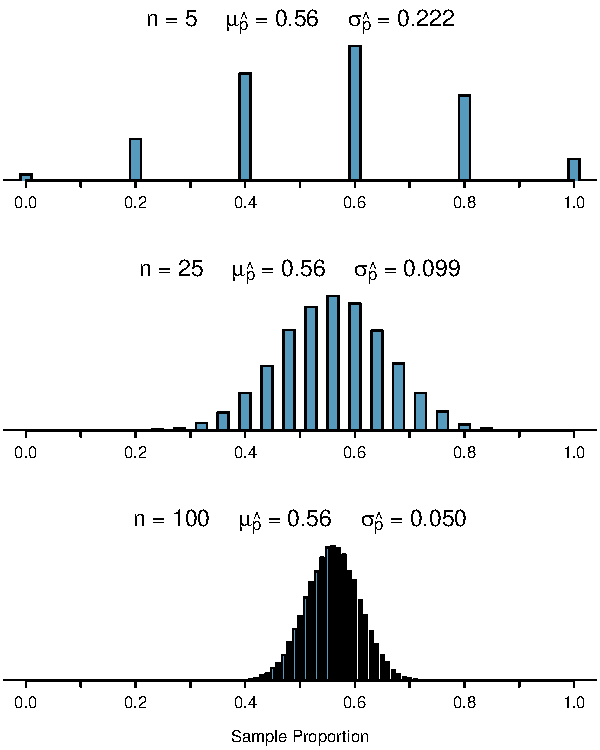
\includegraphics[width=0.67\textwidth]{ch_inference_for_props/figures/sampling_X_prop_56p/sampling_X_prop_56p}
   \caption{Simulations of $\hat{p}$ when the population
       proportion is $p = 0.56$ and for the following sample sizes:
       $n = 5$, $n = 25$, and $n = 100$. The theoretical
       mean~($\mu_{\hat{p}}$) and standard
       deviation~($SE_{\hat{p}}$) is also provided for each plot.}
   \label{sampling_X_prop_56p}
\end{figure}

%\begin{termBox}{\tBoxTitle{Law of Large Numbers for proportions}
%  \hiddenterm{Law of Large Numbers!proportions}
%  When the sample size is large, the sample proportion tends to be
%  a more reliable estimate of the population proportion.}
%\end{termBox}

Next let's consider what happens when we use different proportions.
For this exploration, let's use a sample size of $n = 100$ and
proportions of 0.03, 0.20, 0.50 0.80, and 0.97. The distributions
are shown in Figure~\ref{sampling_X_prop_56p}. Below are key
takeaways from these simulations:
\begin{itemize}
\item When the population proportion $p$ is close to 0 or 1, the
    distribution of sample proportions tends to be skewed. However,
    for proportions relatively far from   gets larger, the
    distribution becomes more symmetric
\item The estimates tend to be less variable when the proportion
    is near 0 or 1, as is shown by their lower variability listed
    in the table.
\end{itemize}

\begin{figure}
   \centering
   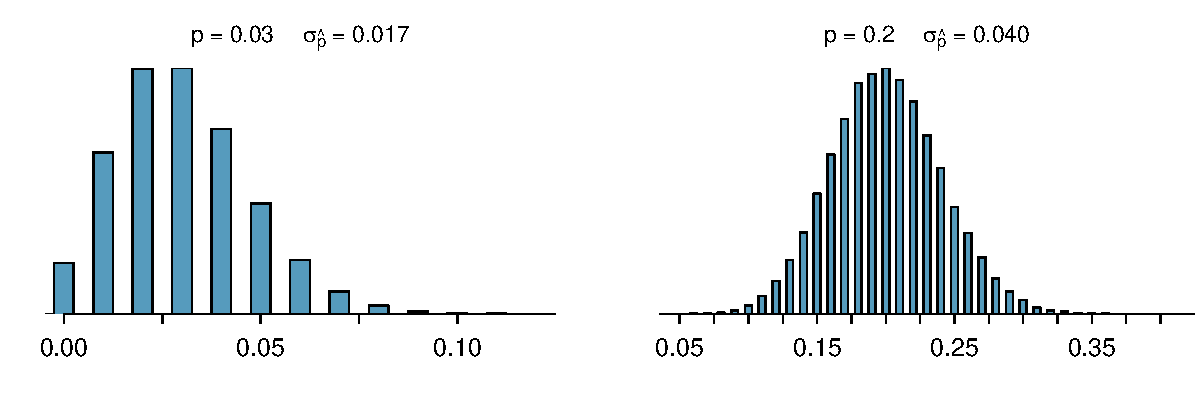
\includegraphics[width=\textwidth]{ch_inference_for_props/figures/sampling_100_prop_X/sampling_100_prop_X_12}
   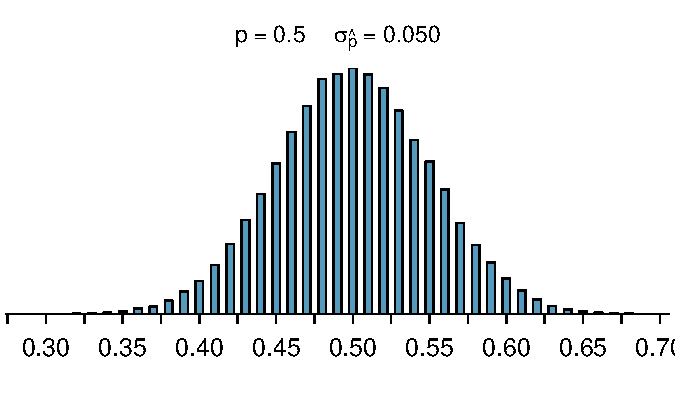
\includegraphics[width=0.55\textwidth]{ch_inference_for_props/figures/sampling_100_prop_X/sampling_100_prop_X_3}
   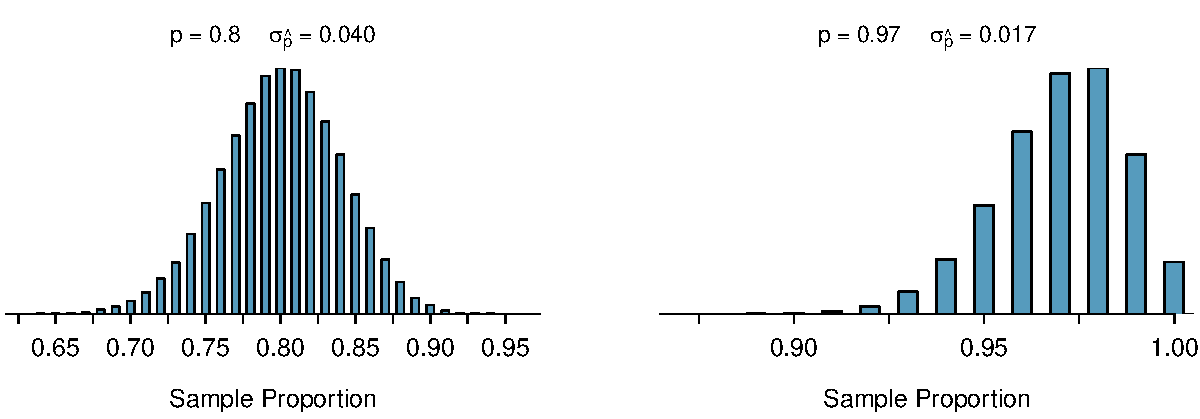
\includegraphics[width=\textwidth]{ch_inference_for_props/figures/sampling_100_prop_X/sampling_100_prop_X_45}
   \caption{Simulations of $\hat{p}$ for different population
       proportions when the sample size is $n = 100$. Each plot
       is centered at the population proportion $p$, and the
       theoretical standard deviation ($SE_{\hat{p}}$) is
       also provided for each plot.}
   \label{sampling_X_prop_56p}
\end{figure}

\Comment{Make sure the plots show $SE_{\hat{p}}$ rather than $\sigma_{\hat{p}}$.}


\subsection{Sampling distributions and the Central Limit Theorem}

In general, when we consider the distribution of a statistic, such as
a sample proportion, we call it a \term{sampling distribution}.
That is, the distribution shown in Figure~\ref{sampling_10k_prop_56p}
is a \emph{sampling distribution} for a sample proportion when the
sample size is 1000 and the population proportion is 0.56.

\begin{termBox}{\tBoxTitle{Sampling distribution}
  The sampling distribution represents the distribution of the point
  estimates based on samples of a fixed size from a certain population.
  It is useful to think of a particular point estimate as being drawn
  from such a distribution. Understanding the concept of a sampling
  distribution is central to understanding statistical inference.}
\end{termBox}

